% Chapter 1

\chapter{Literature Review} % Main chapter title

\label{literaturereview} % For referencing the chapter elsewhere, use \ref{Chapter1} 

\lhead{Chapter \ref{literaturereview}.\emph{Literature Review}} % This is for the header on each page - perhaps a shortened title

%----------------------------------------------------------------------------------------
\section{Behaviour Change Support Technologies}
Research on ubiquitous computing to support behaviour change in a myriad of domains has received a significant amount of attention. There has been an emphasis on the importance of having incentive systems with emotionally engaging and timely feedbacks to persuade people to change their behaviors~\citep{nakajima2013designing}. 

One of the early pioneers to formalize behaviour change technology as an area of research was B.J. Fogg\footnote{http://bjfogg.com/} who coined a term “captology” which is an acronym for \emph{Computers As Persuasive Technologies} (CAPT-ology), with focus on the planned persuasive effects of computer technologies~\citep{fogg1999persuasive}. In persuasive systems, persuasion is intentional and usually implemented through persuasive stimuli; hence providing a system with the ability to persuade~\citep{hamari2014persuasive}. Persuasive technologies have applications in domains such as health-care, education and training, environmental sustainability, etc..

According to~\cite{langrial2012digital}, the evolution of research on behaviour change technologies through the realms of computing research started with digital interventions in early 1990s which were basically for intervening behaviours in the preventive health area primarily through reminders; to persuasive technologies - systems that implement various software functionality that utilize approaches such as social learning or comparison etc; to the current behaviour change support systems (BCSS) which provide models and frameworks for designing and evaluating persuasive technologies.~\cite{Oinas-Kukkonen:foundation} defined a BCSS  as ``a socio-technical information system with psychological and behavioural outcomes designed to form, alter or reinforce attitudes, behaviours or an act of complying without using coercion or deception''.

Separate models (frameworks) to guide the design and evaluation of persuasive technologies have been proposed since models from information systems such as a \emph{Technology Acceptance Model} (TAM) have limitations with regard to understanding the effectiveness of persuasive technologies~\citep{Oinas-kukkonen:psd}. Persuasive technologies' models tend to provide nuanced features and characteristics that define such systems.~\cite{fogg2009behavior} recommended a behaviour model for persuasive design which asserts that for a person to perform a targeted behaviour, he or she must (1) be sufficiently motivated, (2) have the ability to perform the behaviour, and (3) be triggered to perform the behaviour.~\cite{fogg2009behavior2} also recommended a behaviour grid that one can use to design persuasive technologies. In this behaviour grid, persuasive strategies are matched to targeted behaviours. 

\cite{Oinas-kukkonen:psd} extended Fogg's work~\citep{fogg2009behavior} with a more comprehensive model known as a \emph{Persuasive System Design} (PSD) model which suggested three initial steps: (1) analysis of the persuasion context, i.e. with focus on the intent of persuasion and context of use, user, and technology; (2) selection of persuasive features to use; and (3) selection of persuasion strategies to use i.e. whether to use a direct or indirect route of persuasion. The PSD model also outlined 28 design principles discerned into the following five categories: (1) \emph{primary task support}, which includes activities such as, reduction of complex behaviours into simple tasks, guiding the user through experiences while persuade along the way, tailoring of persuasive information to factors relevant to a user group, personalization of content, and self-monitoring for users to keep track of their performance towards their specified goals; (2) \emph{dialogue support}, which includes praises, rewards, reminders, similarity, liking, and social roles; (3) \emph{system credibility support}, which includes trustworthiness, expertise, surface credibility etc; and (4)\emph{social support}, which includes social learning, social comparison, and competition.

An extension to the PSD model was an \emph{Outcome Change} (O/C) matrix of which one could use when analysing an intent of persuasion~\citep{Oinas-Kukkonen:foundation}. The O/C matrix matches the type of change that needs to be applied with a specific outcome. A change could either be of compliance (C) or behaviour (B) or attitude (A), nature. While an expected outcome could be forming, altering, or reinforcing any of the aforementioned types of change. The extended PSD model with O/C matrix is called BCSS as mentioned in the classes of behaviour change systems above. BCSS is considered to be the foundation for studying persuasive systems and it is meant to provide a base for analysis, design, and evaluation of persuasive technologies. The next section highlights how behaviour change technologies have been applied in health domain.

\section{Behaviour Change Technologies for Health}
Health-care providers are eagerly seeking for innovative solutions that could help in monitoring and improvements of the patients' health~\citep{higgins2016smartphone}. Innovative ways to support health promotion and management are in need to respond to the health care crisis as the result of unprecedented increase in prevalence of lifestyle-chronic diseases~\citep{arsand:mobile}. Health-care systems do not have sufficient resources to cope with the increasing burden of chronic diseases~\citep{quinn2008welldoc,arsand:mobile}; hence these innovative ways aim at supporting the advocacy of shifting from physician centred care to patient-centred care~\citep{higgins2016smartphone,korhonen2010personal}.  Literature has demonstrated the dominance of persuasive technologies targeting health behaviour change. For instance one recent systematic review of 95 studies that examined the ability of persuasive technologies to persuade, had approximately included 47 \% studies that  targeted domains of health and exercise~\citep{hamari2014persuasive}. The remaining 53\% was shared by several domains such ecological consumption and/or behaviour (21\%, second highest), education/learning economic (11\%), etc.. Therefore, this indicates that health is an important area of concern when the notion of persuasive technologies comes in mind.

\cite{chatterjee2009healthy} classified three generations  of technological evolution of hardware and software utilized in implementations of behaviour change interventions in health. The first generation started to emerge from 1960's and it was characterized by the prescriptive nature of information flow from physician, health care provider, or technology-based system to a health care recipient. Decades worth of research has shown that phone-based or simple messaging technologies can improve the quality of health care management and clinical outcomes. The second generation is characterized by the descriptive nature of information interaction between a user and the persuasive technologies and examples of such systems include interactive websites, personal data assistants (PDAs) that allow activity recording, and simple sensors that record and report basic health parameters. The third generation extends second generation by providing body-wearable sensors that support advanced health monitoring, use of context-aware computing to determine when to deliver “just in time” messages.  While the second generation utilized PCs and later cellphones, the third generation is dominated mostly by cellphones and ubiquitous computing devices. The future generation is expected to be the one that will entail ubiquitous computing integrated seamlessly into people's daily lives and it will be supported with data mining techniques~\citep{chatterjee2009healthy}.

The first and second generations systems are the ones that have received most appraisal because of existing randomized clinical trials. The evidence of their dominance in public health is demonstrated by the preponderance in publications that report on the use web based interventions integrated with SMS text-messaging on clinical settings. Existing systematic reviews~\citep{cole2010text,fjeldsoe2009behavior,krishna2009healthcare} reported more on the use of SMS reminders and feedbacks on areas of diabetes self-management, smoking cessation, and weight reduction therapy. There are mixed results on effectiveness of cellphone or other ICT interventions on weight loss production. For instance one randomized control trial (RCT) that was carried out for a period of two years~\citep{svetkey2015cell}, revealed that a control group that was supplied with only pamphlets materials with health information reduced weight significantly compared to two intervention groups; one group using a mobile app, and the other group using both a human coach and a mobile app. In addition to mixed results that are often found in such clinical trials.~\cite{cole2010text,kaplan2006can} also pointed out that the design of such interventions may not scale well to specific demographics within resource constraint contexts. From persuasive technology literature perspectives it has also been observed that there is a gap between research in persuasive technologies and RCTs in public health settings. Literature from public health is being criticized for lacking adequate information on how individual systems were designed as such systems are usually poorly described since most work is being published by public health practitioners without involvement of computer scientists~\citep{Oinas-Kukkonen:foundation}.

Persuasive technologies provide means to personalize health information. Personalization of health information is advocated within public health domain as it allows consideration of individual needs of a person and it also gives a targeted person, a  sense of control over their healthcare~\citep{mccallum2012gamification}. This research was focusing on personalized technologies that support data collection and feedback for an objective of health persuasion. These systems are referred to as wellness applications or personal health informatics. 
\section{Personal Informatics for Health Behaviour Change}
Personal informatics is a class of interactive applications that support users to improve self-awareness of various facets of their lives by providing technological means to support in collection and analysis of personal data related to habits, behaviours, and thoughts~\citep{li2011personal,li2012personal}. A personal informatics system augments the activity of \emph{self-reflection} by complementing individuals in storing events that can hardly be recalled due to limitations in humans' memory~\citep{li2010stage}. The goal of personal informatics systems is to support individuals in having a better understanding of their lifestyle or behaviours. These systems are important in promotion of positive behaviors in a myriad of domains such as healthy lifestyle~\citep{korhonen2010personal}, recycling~\citep{comber2013designing}, energy conservation~\citep{seligman1977feedback}, etc. 

Research on personal informatics systems tends to focus on, effective ways of, collecting users' personal data in an effortless manner, and supporting for self-reflection through feedback mechanisms~\citep{li2011understanding}. Data collection is usually supported with context-aware sensors and self-reporting mechanisms. Sensors may be coupled together with a computing device for both analysis and feedback or may be coupled in an external device that transfer data through either wireless means or data cables, to a computing device responsible for analysis and feedbacks.~\cite{nakajima2013designing} proposed the use of a metaphor ``\emph{ambient persuasive mirrors}'' to describe displays that can support self-reflection of one's own behaviour. These mirrors may be multifaceted and may apply transformation and integration of data from other sources, and their implementation can be on, personal mobile devices~\citep{klasnja2009:using} or shared public interfaces~\citep{lin2006:fish}.

Personal informatics systems can be applied in prevention of onset of chronic conditions by motivating healthy individuals to change their lifestyle. Specifically, these systems promote behaviours that are beneficial in, preventing weight gain or weight loss. These systems operate by facilitating logging of data related to personal behaviour. This act of behaviour logging can also be beneficial in self-management of chronic conditions as it provides support for a self-monitoring task. Self-monitoring is very essential in supporting cognitive behaviour therapy (CBT) within public health settings~\citep{mattila2008mobile}, especially for individuals who are clinically obese~\citep{nih2000practical}. Health self-management programs usually ask participants to keep records of their activities, physiological variables and other health-related data; personal informatics applications can make this process simpler and easier~\citep{medynskiy2010salud}. For instance participants may record their daily calorie intake,and then have graphs that show trends of how far they have gone with reducing their intake. The essence of self-monitoring is to promote self-awareness of one’s behaviour. That consciousness is fostered through behaviour observation. And behaviour observation can be achieved through behaviour recording. Therefore, collection of data on one's own behaviour can viewed as an important self-assessment approach for helping patients to observe and react on their own behaviours~\citep{rapp2014meaningful}. This implies that with a self-monitoring system or app, processes of recording and self-reflection are simplified through technology. 

Literature presents a wide range of mobile phone based personal informatics systems for promotion of physical activity, blood glucose monitoring, and healthy eating. Some of these are specifically for chronically ill patients e.g. ``Few Touch Application'' which targeted individual with  \emph{Type 2 Diabetes}~\citep{arsand:mobile}, and a system described by \cite{arteaga2010:persuasive} that targeted teenagers with weight management issues. There also exists systems that target general populations, and used for promoting healthy eating habits and engagement in physical activity e.g. Fish'n'Steps\citep{lin2006:fish}, UbiFit Garden\citep{klasnja2009:using}, Wellness diary\citep{mattila2008mobile}, ActivMon\citep{burns2012using}, PmEB\citep{lee2006pmeb}, iCrave\citep{hsu2014persuasive}, etc. 

Models and frameworks for understanding both physical, social, psychological needs of users within the context personal informatics have been vastly explored.~\cite{kamal2010understanding} presented a framework for designing a system that integrates online social networks and personal informatics to promote positive health behaviours. The framework was informed by theories from both health behaviour change and social networks.~\cite{li2010stage} proposed a model for understanding how people use personal informatics by transitioning between the following five stages: preparation, collection, integration, reflection, and action. The importance of identifying barriers at each stage is emphasized since these barriers may also cascade to later stages to hinder the process of data collection and self-reflection. In order to address cascading barriers, it was recommended that the design process should be carried out in an holistic approach that involves iterations between stages. The aforementioned model aimed at helping with the process of designing a personal informatics system. There are also studies that have explored design implications for data logging systems that support self-reflection. For instance ~\cite{li2011understanding} highlighted that such tools should be designed to address six questions that users ask themselves when engaging with their personal data; these questions are based on, status towards achieving their goal, history for the purpose of discovering patterns that are crucial to the preferred behaviour, formation of goals to facilitate in attaining a preferred behaviour, discrepancies between their behaviour and goal, context of past behaviour in order to discover patterns, and discovering of factors that may affect their behaviours. The aforementioned questions are asked in two phases of which the user alternates in the course of using a personal informatics systems. The two transition phases of behaviour change are self-discovery and maintenance. In the self-discovery stage individuals collect a lot of data they can use to discover patterns in their behaviours. After discovering of a pattern they can move to the maintenance stage. The maintenance stage entails setting of a personal goal and monitoring of a status towards achieving that goal. Users don't stay permanently in one phase. It is possible for an individual in the maintenance phase to go back to discovery phase if there is a new unknown pattern that has emanated and appears to affect their behaviour. Another study by~\cite{macleod2013personal} suggested factors that drive motivation of chronically ill people in engaging with their personal data as; curiosity, and self-discovery of what is happening in their health.

The most recent model to help in understanding how people use personal informatics systems, suggested that these systems are meant to be fully integrated into people's daily lives~\citep{epstein2015lived}. This model extends~\cite{li2010stage}'s model, by splitting the preparation stage into \emph{deciding to track} and \emph{selecting tool} processes; and combining collection, integration, and reflection into tracking and acting. This model also includes further stages beyond tracking and acting and these were lapsing, and resuming tracking.  From lapsing, issues that contribute to discontinuation or intermittent usage are explored, while in resuming tracking, issues such as switching of tools, incorporation of previous history/data while resuming to use are explored on this stage.  

The last stage of the \cite{li2010stage}'s model suggests on providing guidance to an end user towards an action. However, guiding an end user through an action/acting stage for the objective of minimizing barriers in execution of the action stage, can be perceived as an attempt to nudge individuals towards certain behaviours. There has been a debate from HCI research community of whether behavioural nudges are ethically accepted or not as some researchers are proposing a more neutral approach while others recommend application of intervals of behavioural nudges upon tracking (collection and reflection) activity.  For instance,~\cite{munson2012mindfulness} advocates that the focus on personal informatics  should be towards enabling end users to better know owns behaviour instead of applying behavioural nudges, and suggests that adoption should be voluntary. Also in \cite{epstein2015lived}'s model it is highlighted that sometimes people use personal tracking systems for other reasons beyond behavioural change goals such as instrumental benefits (i.e. to get rewards from location trackers like Foursquare), or out of curiosity. However, \cite{epstein2015lived}, still  shows that in most usage that is related to health domain i.e. in physical activity, behaviour change goal is a dominant motivational factor~\citep{epstein2015lived}; hence suggestions on what actions an end user should take are inevitable. In addition to this, technology is considered not to be neutral~\citep{Oinas-kukkonen:psd}. Technology has a capability of presenting social cues that trigger emphatic responses from humans~\citep{foggpersuasivebook}. If no action is recommended, still an action can come from within a person using the system as the result of self-reflection. According to~\cite{fogg1998persuasive} cited in~\cite{Oinas-kukkonen:psd}, intent of persuasion can originate from either of the three sources which are: (1) from the people who create or produce interactive technology; (2) from people who give access to or distribute the interactive technology to others; and (3) from the people who use or adopt an interactive technology. The intent of persuasion may also come from within the person using a system that does not recommend or suggest any actions. The persuasion may be as the result of cognitive dissonance after self-reflection. People like their views of the world to be consistent and It also assumed that people always make rational and informed decisions~\citep{Oinas-kukkonen:psd}. By using personal informatics, individuals' decisions can be improved by being be able to see the discrepancies between their desired behaviours versus their performance~\citep{comber2013designing}. If there are inconsistencies, then a cognitive dissonance is introduced which may mediate a change of attitude or behaviour in order to restore consistency between beliefs and actions~\citep{Oinas-kukkonen:psd}. Therefore, an act of tracking(collection and reflection) itself can mediate a behaviour change through cognitive dissonance. The motivation of usage of personal informatics in domains such as health and finance has been found to be related to a behaviour change goal~\citep{epstein2015lived}. From this perspective, a basic personal informatics system with simply self-monitoring support can be viewed as a persuasive technology in contexts such as personal health and finance, because of its ability to trigger cognitive dissonance which can be considered as a persuasive stimulus. Knowing one self can be important in adoption of a better lifestyle. For instance one study found the use of pedometer alone (without other motivational affordances) increased physical activity by about 1 mile of walking per day~\citep{bravata2007using} cited in ~\cite{albaina2009flowie}.  

One of the common strategies to make cognitive dissonance more salient involves setting of personal health goals, which has been recently used in many developed systems i.e. Few Touch Application~\citep{arsand:mobile}. This idea is derived from a goal setting theory~\citep{strecher1995goal}. An example of a goal could be to walk for at least 30 minutes every day or to increase the number of times a person eats fruits and vegetables or to reduce the amount of starch in a meal. One way of tracking progress towards the goal is through feedbacks that may simply implemented through SMS, or some sophisticated visualization approaches. The common data visualization techniques consists charts and graphs. Beyond charts and graphs, the use of metaphors that requires users to take care of virtual pets is becoming prevalent as a means to emotionally engage users with their personal health data concerning physical activity and diet~\citep{lin2006:fish,albaina2009flowie,klasnja2009:using,pollak2010s,nakajima2013designing}. The use virtual pets has been used in promotion of behaviors such as drinking of water~\citep{lessel2016watercoaster},recycling behaviours~\citep{comber2013designing}, reduction of CO2 emissions and proper tooth brushing~\citep{nakajima2013designing}, etc.. The most popular virtual pets are the ones that use plants or fish metaphors and these metaphors have shown promising results in supporting end users with their motivational needs. For instance~\cite{nakajima2013designing} described a situation of where participants felt guilty when their trees died. Another example is that of a Fish'n'Steps~\citep{lin2006:fish} application of where some of the participants were saddened when their fish appeared to be sad because participants had not walked enough steps. The aforementioned examples demonstrate how the use of virtual pets could invoke end users' emotional attachment with their virtual pets. Utilization of informal art displays in promotion of physical activity is also reported in literature~\citep{fan2012spark,nakajima2013designing}. 

The motivational paradigms in persuasive technologies have also been extended to exploration of systems with social incentives that entail social collaboration, social interactions, social support, and competitions or social comparison for the purpose of enhancing engagement of end users~\citep{ploderer2014social,chen2016social,epstein2015nobody,reno2016matters}, and this brings the notion of gamified personal health informatics~\citep{lin2006:fish,chen2014healthytogether,han2014designing}. Cooperation and competition features have been found to be among effective incentives in pervasive fitness applications~\citep{chen2016social}. Also the use of social influence through social networks integrated with personal informatics is very promising. For instance in a BinCam~\citep{comber2013bincam,comber2013designing} system they used social norms influence as a motivation strategy to encourage individuals within a household to be more conscious of their recycling behaviours by comparing themselves with other households.~\cite{bales2011interpersonal} proposed the idea of interpersonal informatics systems that aim at making the social influence more salient to individuals using the personal informatics. The authors of the aforementioned paper argue that personal choices are also as the result of the influence of social networks in which one participate. The essence of the aforementioned approach was to support individuals in becoming more aware of how those around them affect their habits, beliefs, and health. This idea of social influence is also explored by~\cite{ploderer2014social} using the notion social interaction that ranges from minimal social traces of other people's activities to rich social interaction via social media, to systems that focus on collective use rather individuals. Therefore, sharing of personal data is an important catalyst for social interactions. The reason of why people share their personal data is to receive emotional support and communicate their identities~\citep{epstein2015nobody}. However, sharing systems in personal informatics need to be designed to support users in being able to present themselves in a way that they can receive positive social support or encouragement from their appears since fear of misrepresentation can hinder utilization of social support~\citep{ploderer2014social,epstein2015nobody,reno2016matters}.

Despite such tremendous development in the field of personal informatics for health promotion, most of these systems are designed for the developed world context. Even existence of randomized clinical trials on utilization of a simple technology such as SMS is largely dominated by countries from developed world~\citep{cole2010text}. From HCI point of view, engagement with personalized systems is currently considered to be more personal from data collection to reflection processes. These applications are personal in the essence of ownership of hardware, applications, data stored in application, and the process of interacting with a system for both data collection, and reflection. The technology interaction context of the existing applications may not be versatile in developing world perspective especially in low income communities of where  both sharing in usage of technology and indirect usage through intermediary or proxy users are common~\citep{kaplan2006can,sambasivan2010}. HCI in the developing world is a complex relationship between technology, multiple users, indirect stakeholders, observers, and bystanders~\citep{parikh2006}. An interaction model that assumes one phone/device one person might not always be feasible in such contexts. Also in many contexts, interaction with technology may not be direct; intermediation by another person occurs when the primary user is not capable of using a device entirely on their own~\citep{sambasivan2010}. For users with limited technology literacy or education, direct access to a user interface might not even be feasible~\citep{parikh2006}; hence intermediation might be the only means for these people to be able to perceive the benefits derived by the proliferation of mobile phones or any other ICTs. While many people in developing world context might lack textual and digital literacy, low-income communities are diverse and often there are some members who have competent skills to operate technology \citep{sambasivan2010}, and these people may be able to help others to benefit from technology usage.

The complexity of usage through intermediaries is beyond help on the spot \citep{sambasivan2010}; hence it cannot be merely solved by endeavours to simplify the user interface. In exploring of why intermediated technology use is beyond help on spot, one has to look at the notion of collectivist societies. In collectivist societies, people engage in tasks in group formation. For instance, India is considered to be a collectivist society of where individuals are prone to group orientation towards tasks~\citep{parikh2006}. This encourages usage of technology through human intermediaries. In such usage at least two users are involved in one interaction process. There is much more complexity on factors that influence intermediated technology use ; hence it cannot be simply explained by existing interaction models from computer supported collaborative work~\citep{parikh2006}. Sukumaran et al (2009) emphasizes the importance of having a better understanding of locally specific interaction models to address culturally influenced issues in using information technology throughout the developing world. Intermediated interaction in an example of such interactions that needs to be clearly understood.

In the context of personal informatics, frequency of usage may vary among different domains, with the ones targeting physical activity being used more frequent (on daily basis), while other domains usage is from once a week and beyond~\citep{epstein2015lived}. Therefore, for a context where an end user needs help, motivation to use, is no longer just for this user but also it has to consider the person helping. This research was particularly focusing on how a personal health informatics system  designed for a personal use can be adapted in the context where two sets of users are being involved in an interaction process (the first one being a beneficiary of that technology, meaning a person receiving help on an interaction task to both collect and self-reflect on their personal data, while the second one is an intermediary user, a person providing assistance to a beneficiary user). 

The next section highlights the broader view of intermediated technology use in the context of both developing and developed world communities.  

\section{Intermediated Technology Use}
The role of human intermediaries within the context of ICTD has well emphasized as to be beyond that of translators of policies to the ground level~\citep{bailur2010liminal}. According to~\cite{heeks1999tyranny}, cited in~\cite{bailur2012complex}, human intermediaries bridge a gap between what the poor have and what they would need in order to use ICTs. An example of scenarios of where intermediaries have been of great value is that public access venues (PAVs) such as telecentres. Without the presence of these facilitators in PAVs, the groups that are excluded from access due to their age, socio-economic status, level of education/literacy, gender, disability or caste are more likely to face barriers in accessing information~\citep{ramirez2013infomediaries}. Therefore, human infrastructure within ICTD context plays an instrumental role in facilitating information and communication access in low income communities~\citep{sambasivan2010human}.
It has been suggested on literature that one of the factors that contributed to failure of past PAVs initiatives is lack of understanding of position and motivation of intermediaries~\citep{bailur2010liminal}.
 
Human factors that affect and shape the outcome of facilitating information and communication access through human intermediaries have been explored. For instance~\cite{bailur2010liminal} used structuration theory\citep{jones2008giddens}, to understand the contradiction and conflict of intermediaries on interacting with their different networks i.e. how they play a liminal role with stakeholders of PAVs and multimedia centres (i.e. NGO or government, donor agency on one side and community on the other side).~\cite{bailur2012complex} argues that PAVs' intermediaries should not be taken for granted in the space of ICTD because they play a complex position of brokers and translators as they assume multiple identities to different stakeholders of which their roles are constantly negotiated and performed within these multiple constructed networks. Another study is by \cite{ramirez2013infomediaries} which investigated how human factors such as empathy and technical skills of infomediaries influence the outcomes of the process of infomediation to users at PAVs. 

The ecosystem of utilization of intermediaries in PAVs or other community centres has also been examined through lens of HCI. Focus on HCI has been on engagement of all layers of users involved in intermediated interactions.~\cite{parikh2006}'s study in India provided a taxonomy of intermediated information tasks from HCI perspective;  of which  different modes of access were distinguished, and each one of them was suggested to have its own design requirements. These modes of access were: (1) cooperative, of whereby several users fairly collaborate without domination by a single or fewer users; (2) dominated interactions, of whereby users collaborate but they is one or fewer users who dominate others in manipulating user interfaces; (3) intermediated interactions, this whereby the first user manipulates interfaces while the  rest of users are just observing what is happening; and (4) indirect interactions, of where one or multiple users are being assisted to interact with a system without being being present or observing while manipulation of user interfaces is taking place. ~\cite{sukumaran2009intermediated} conducted an experiment that investigated how social prominence of an intermediary versus technology in a computer kiosk affects perceived information characteristics and attitudes towards an interaction by a beneficiary user/secondary user and found out that when the technology was more visible and an intermediary did not monopolize access (situation of social equality), beneficiaries tended to feel more engaged and positive. 

Although intermediaries in public access venues are considered as policy implementers on the ground level through working with communities, their position is very complex as they are the bottom of the hierarchy but they are also perceived not to be part of the community; hence they cannot specifically identify with a certain group since their roles are adapted according to circumstances~\citep{bailur2010liminal}. Motivation of intermediaries in this context of PAVs is negotiated relative to their particular network. A different ethnography study by~\cite{sambasivan2010}, explored the dynamics of intermediation beyond public access venues (\emph{i.e in inherent home, or community settings that involve neighbours and family members as intermediaries} --these intermediaries are more embedded to the community as they are considered part of it). \cite{sambasivan2010} presented three distinct forms of intermediated interactions: inputting intent into the device in proximate enabling, interpretation of device output in proximate translation, and both input of intent, and interpretation of output in surrogate usage. This study also highlighted: (1) social mediators of motivation for intermediation such as interpersonal trust or prior social rapport, a give and take economy, social structures (i.e. access constraints due gender, economic status, tendency of reliance on others, etc.), etc.; and (2) design implications to enhance engagement of users (primary and secondary users) such as : reorientation of technology  to allow sharing between primary and secondary users for asymmetric engagement; and supporting persistent storage of information for retrieval at later stages by beneficiary users. The study also proposed that measurement of use should go beyond ownership to also consider those who benefit without direct usage. 

The concept of informal help in technology use within family and social network settings is not an exclusive  phenomenon of developing world only; it is present in developed world as well. For instance ~\cite{poole:chh} cited in~\cite{katule2016leveraging} examined the dynamics of computer help-seeking and giving behaviors in the context of family and social networks settings, their findings indicated that an important factor that  encourages help-seeking behaviors is availability of unlimited help provided as a part of a longer-term relationship, while in the case of help-givers, they are motivated by a sense of being accountable to their family members and friends.

In the next subsection it is discussed of how intermediaries have been used in other health behaviour change interventions in the context of developing world and what is the gap from literature.

\section{Intermediaries in Supporting Health Behaviour Change}
In the context, of health behaviour change, typical examples of human intermediaries is on utilization of community health workers who provide access to health information to less privileged individuals in resource-constrained environments.  In many ICTD projects, CHWs, access health information on behalf of communities in which direct access to health resources is not possible, and are an effective bridge between communities and government-based resources~\citep{katule2016leveraging}. One project in India used community health workers (CHWs) -referred to as  ASHAs (Accredited Social Health Activists), of where these ASHAs were empowered with mobile phones that contained persuasive messages. These messages gave ASHAs credibility in persuading pregnant and postnatal women together with their relatives on maternal health issues~\citep{ramachandran2010mobile,ramachandran2010research}. Most of these ASHAs are women.

One project in Lesotho~\citep{molapo2013software}, empowered rural health trainers with a software application for creation of digital  training  content, voice-over images  that can be used by low-literate CHWs to train clients in the villages. While the main objective of these podcasts was for training purposes, upon CHWs showing them to their clients, there were unintentional persuasive effects that motivated these clients to get tested for diseases such as tuberculosis.

A study by~\cite{kumar2015mobile} in India, used a feminist reflexivity lens to study how patriarchal structures and social conventions constrain women in accessing maternal health information, and how these women leverage help from intermediaries within communities to navigate their way out. The study further highlighted different groups of intermediaries who facilitate dissemination of information and examples of these intermediaries include but not limited to mobile shop owners, children and youth, and ASHAs. Another finding from that study is that even ASHAs may also face constraints on the process of transferring mobile media to their phones; hence they tended to seek help from their family members. Another observation was on technology access in patriarchal families of where access to cellphones was mostly dominated by men. In such contexts children appeared to have free access to their fathers' devices; hence these children were using the same devices to facilitate their mothers with information access.~\cite{vashistha2016mobile} conducted a fourteen (14) weeks experiment to compare three distribution channels in dissemination of mobile videos on maternal health; mobile shop owners, laptop owners, and ASHAs. Both of the three distribution channels were found not to be very different, however, ASHAs were found to be more effective in distributing videos to the people who where need or demand of such videos.

In the aforementioned projects that utilize CHWs, these CHWs were acting as human access to information that had a persuasive effect. A challenge with utilizing CHWs is that their availability is limited to fewer visits in intervals of weeks or months; hence may not be suitable for a technology such as a personal health informatics of which its beneficiaries may need to engage with a it more frequent. Also other forms of distribution and viewing have limitations as it was found in~\cite{vashistha2016mobile}'s study that dissemination decreased over time, therefore, it was  suggested an exploration of alternative mechanisms  to extrinsically motivate intermediaries and viewers for broader video distribution.

In the context of children and youth within family settings, one may argue that their innate tendency to care for members of their families or communities may be a sufficient motivational factor for sharing health information, however there may be some limitations to that approach considering the fact that a personal health informatics may require frequent engagement, and without intermediaries having an interest in the system, it is not possible to have sustained usage. A study by~\cite{epstein2015lived} found that users of personal informatics that target health domains such as physical activity have tendency of using them more frequent (at least once per day) compared to personal informatics targeting other domains. Introducing such a system in an ecosystem of intermediated technology use can introduce the following implication on its utilization; there is a possibility that people who are less familiar with such systems to seek help more often. Dependence on  an innate intrinsic motivation of intermediaries alone may hinder availability of such a system to beneficiaries. The outcome of this is that there will be an intermittent usage which may have an impact on self-reflection, therefore, introducing a bottleneck in persuasion. The caveat of relying on natural intrinsic motivation of children to help their parents is also exhibited in a study by~\cite{kiesler:twi} about informal help, of where parents reported  to be skeptical in seeking help from their children in order to avoid negative experiences (i.e annoying their children because of asking for help more often). This proves that for systems such as personal health informatics of which help may be solicited more often, there is a need to explore on motivation techniques to enhance user experience of intermediaries. In the next section, the discussion is centred on a theoretical foundation on, motivation and user experience strategies that were applied at later stages of this study in order to encourage utilization of a personal health informatics through family intermediaries. This study puts an emphasis on engaging intermediaries to become part of that ecosystem. Motivation is explored through the lens of self-determination theory.
\section{A Self-Determination Theory Approach to Motivation}
Motivation is categorized into intrinsic motivation (i.e. inherently embedded with ones' values and goals), and extrinsic motivation (i.e. doing something because of expecting some external outcome)~\citep{ryan2000intrinsic}. Therefore, the locus of control is internal to the person in intrinsic motivation while in extrinsic motivation the locus of control is external to the person~\citep{lee2015:relating}.

Self-determination theory (SDT)\citep{deci1985:intrinsic}, a well grounded theory of human motivation, is concerned with how individuals develop interest to engage with certain activities that were once considered uninteresting~\citep{ryan2000intrinsic}. SDT has two sub-theories namely: (1) cognitive evaluation theory, which focuses on supporting of the certain basic psychological needs in order in increase enjoyment of an activity or task; and (2) organismic integration theory (OIT), which focuses on the process of internalization of a regulation of a behaviour through extrinsic motivations. The OIT further discerns extrinsic motivators that can foster intrinsic motivation from extrinsic motivators that can harm intrinsic motivations~\citep{ryan2000:self,lee2015:relating}.

Cognitive evaluation theory suggests that an intrinsically motivated activity is performed out of satisfying some psychological needs, therefore, for an uninteresting activity to become interesting through external rewards, social factors must provide support for the following three basic psychological needs; competence, relatedness, and autonomy~\citep{ryan2000intrinsic}. Autonomy deals with volition in initiation and regulation of a behaviour. It also emphasizes on the importance of individual's freedom to choose their own identity to represent oneself.  Autonomy gives individual freedom to choose when and how, they want to initiate a behaviour. Competence emphasizes the need for individuals to be presented with challenges that give them a chance to sharpen or develop skills that match presented challenges. Challenges should not be too difficult or too easy to accomplish~\citep{zhang2008motivational,colineau2011motivating}. This process of providing challenges is appropriate for ones' health psychological development and  overall well-being~\citep{zhang2008motivational}. Competence has a tendency of improving perceived enjoyment provided that there is a guarantee of autonomy~\citep{forde2015informational}. Therefore, in the absence of autonomy, support for competence may not lead to positive outcome on intrinsic motivation. Relatedness is the desire by individuals to feel a sense of belongingness. This implies people enjoy to be connected to others.

The premise of self-determination theory is that a behaviour that is externally motivated can become internalized~\citep{ryan2000intrinsic}.
Organismic integration theory stipulates that different levels of internalization for self-regulation of uninteresting but important activities to become interesting, of which these levels are classified into four stages namely; (1) external regulation, (2) introjected regulation, (3) identified regulation, and (4) integrated regulation~\citep{ryan2000intrinsic}. The four distinct levels of internalization are shown on Figure \ref{figure:oit}. In external regulation, individuals self-regulate because of an external outcome such as contingencies of, rewards or punishment. This similar to conditioning of where a good or bad behaviours have their respective contingencies of rewards and contingencies of punishment. In introjected regulation, individuals self-regulate as an attempt to raise their self-worth with respect to others. Therefore regulation is as the result of ego involvement. In identified regulation, individuals have put value into an activity, therefore, they try to self-regulate an activity because they consider it as important probably for achieving a much broader goal; while in integrated regulation, individuals have fully assimilated the self-regulation to their core values and beliefs.  Integrated regulation shares values with intrinsic motivation although it is not intrinsic motivation since its self-regulation is due fulfilment of an external outcome while in intrinsic motivation self-regulation of an activity is as the result of an activity itself being interesting~\citep{ryan2000intrinsic}. It is possible after doing an externally motivated activity for so long individuals may start to enjoy the activity itself regardless of its external outcome, then at this level the activity has already become intrinsically motivated. The internalization process is governed by social and environmental factors of which individuals function~\citep{ryan2000:self,lee2015:relating}.
\begin{figure}[htbp]
  \centering
    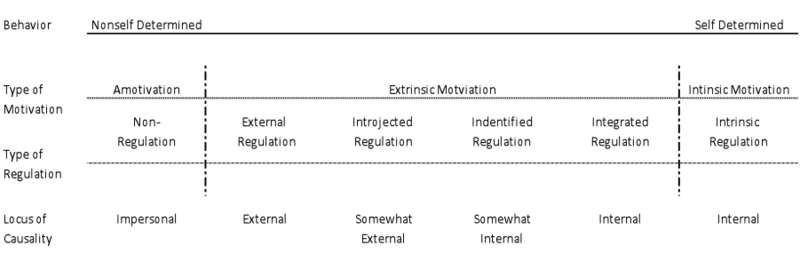
\includegraphics[width=0.8\textwidth]{Figures/oit.png}
    \rule{35em}{0.5pt}
  \caption{Organismic Integration Theory~\citep{ryan2000intrinsic}}
  \label{figure:oit}
\end{figure}

SDT has been used to understand motivation on various activities or behaviours such as; gaming~\citep{ryan2006:motivationalpull}, physical activity~\citep{power2011:obesity}, tobacco cessation~\citep{williams2006:testing}, energy saving~\citep{webb2013:self}, etc. This study brings the motivation pull of gamification in encouraging intermediaries to assist in utilization of personal health informatics. In the next section, gamification is discussed from perspective of self-determination theory.
\section{Self-Determination Theory Support in Gamification}
In order to understand why gamification may be important in intrinsic motivation, one has to understand about motivational triggers behind games.~\cite{knaving2013designing} framed the concept of games in-line with play and fun of where they conceptualized the terms as follows: (1) \emph{fun} is a rewarding and developmentally appropriate process necessary for survival as it imparts humans with skills, knowledge, and social cohesiveness; (2) \emph{play} is a voluntary engagement to an activity in order to have fun and feel pleasure; and (3) \emph{games} is a formal play that is bounded by rules. 

Games have defined goals and immediate feedback on progress towards goals (support for flow) and these are important mediators of optimal experience in play~\citep{knaving2013designing}. One online survey with (N=429) found that social play, relatedness during game play, and flow were some of the factors that were positively associated with players psychological well-being~\citep{vella2013positively}.~\cite{ryan2006:motivationalpull} investigated motivational pull behind video games using self-determination theory and found that needs for autonomy, competence, and relatedness independently predict enjoyment and future game play. The importance of providing support for the three basic psychological needs has been emphasized  by situating the needs into motivational affordances to use ICTs with an objective of fostering motivation in usage of ICT systems~\citep{zhang2008motivational}. 

\cite{nakajima2013designing} argue that we should design systems to mimic the techniques used in games to build emotionally engaging persuasive systems. The motivational aspects of gaming have attracted researchers to explore their usage beyond gaming context and this has resulted to the advent of phenomena such as serious games and / or gamification. Gamification is the use of game design elements in non-game context~\citep{deterding2011game}. Gamification tends to invoke users’ intrinsic motivation through gameful experiences and affordances~\citep{hamari2014persuasive}. Gamification is used outside game context to increase interest on uninteresting but instrumental activities (i.e. physical activity, crowd-sourcing tasks such as image annotation etc.). A systematic review on peer reviewed studies found that gamification provides positive effects and these effects are highly dependent on both the context in which gamification is implemented and the users using it~\citep{hamari2014does}. Extrinsic integrated games have a practical advantage of having patterns that may scale well to different domains while for intrinsically integrated games scalability may be a problem and in practice it is much harder to design an intrinsically integrated game for each domain~\citep{preist2015use}.

The most popular extrinsic motivators in gamification are points, leader boards, achievement badges, levels, story theme, clear goals, feedback, rewards, progress, and challenge~\citep{hamari2014does}. There are different schools of thought on whether gamification itself is a game or not. Most debates are centred around what a typical game entails (i.e. presence of rules, meta-games, immersion, voluntarism in their adoption, etc.)~\citep{seaborn2015:gamification}. According to~\cite{deterding2011game}, users of gamification can socially construct a meaning of whether they perceive gamification as a game or not. The paper further argues what can be experienced in gamification can be termed as a gameful experience with an experiential ``flicker'' between gameful, playful, and other modes of experience and engagement. This means that users could perceive a gamified tool as a game or they could consider it as a tool that is instrumental for achieving a certain objective. For instance while users use a specific tool to achieve something, there is a possibility of the same people experiencing enjoyment from gameful or playful experiences.~\cite{seaborn2015:gamification} argue that the goal of gamification is different from games, therefore, it should rather be considered as an act of integrating user experience to an activity outside game context.~\cite{knaving2013designing} emphasized that while using gamification, the main activity being promoted should remain salient without being overshadowed by gamification; hence they recommended that designers should strike to balance between preservation of an activity being promoted through gamification and designing for playfulness. The goal of gamification should be to impart knowledge about the main activity being promoted; hence a design strategy should be to support both play and internalization.

\cite{sailer2013:psychological} used self-determination theory to understand the motivational pull of game design elements that can be used in non-game contexts of which their research attempted to provide examples of matching game elements to motivation mechanisms; for instance badges can be used to foster a sense of competence, while a leader board can be used to foster a sense of relatedness as it puts emphasis on collaboration among members of different teams. The use of gamification is influenced by social factors such as social influence, recognition, reciprocal benefit, and network exposure; hence it is important to have a community of people who are committed to the goals that the gamification promotes~\citep{hamari2013social}.

\cite{mekler2013points} conducted a study to evaluate if gamification harms intrinsic motivation. Gamification was added to an crowd image annotation tasks. In that study it was found that gamification can increase engagement but intrinsic motivation didn't change as it was not different from the control group. Depending on how a gamified system has been designed, it can either foster or hinder internalization of regulation that is externally rewarded. One way to foster intrinsic motivation is to ensure that gamification provides an optimal internalization (identified or integrated regulation).

There are some suggestions of which one could use gamification to promote motivation towards optimal internalization. An example of such a suggestion is to to make gamification meaningful. An experiment that examined facilitating contextual factors that can foster internalization of regulation of a behaviour, found out that the factors such as framing the task with a meaning (providing a meaningful rationale), being sympathetic about behaver's  feeling, and conveying choice fostered integrated regulation~\citep{deci1994facilitating}.~\cite{nicholson2012user} presents a framework for meaningful gamification that put the user at the centre. The framework was inspired by organismic integration theory explained above, situational relevance and situated motivational affordance, universal design for learning, and player generated content. An example of meaningful gamification, is that of where users are convinced that what they are doing is not just for the sake of playing a game but rather it has a contribution to a good cause. For instance, ~\cite{mekler2013points} they had used points and leaderboard to encourage participants in image annotation tasks and found that even though gamification didn't harm intrinsic motivation but it had affected the quality of image annotation as participants were focusing on completing more tasks in order to advance in gamification. The same experiment was repeated except this time it had included gamification with meaningful framing of where participants in the meaningful framing were informed that their tags would help improve computerized affective image categorization and hence contributing towards an advancement in science. This resulted into better quality tags produced by participants in the meaningful framing condition~\citep{mekler2013disassembling} compared to participants in gamification without meaningful framing. In the context of this research it was hypothesized, pairing an intermediary and beneficiary that have a good social relationship would give intermediaries a good cause as they will be helping people they care about; hence it was anticipated that this framing would make the collaborative gamified system to be perceived as meaningful.

The next section presents utilization of games and gamification in health interventions and what is lacking in literature as far those interventions are concerned with regard to supporting utilization of personal health informatics through intermediary users.

\section{Games in Personalized Health Interventions}
Following the diffusion of video games in many digital devices of which these games are solely used for entertainment purposes, there is an increasing interest on the potential of such entertaining platforms in influencing positive changes in health behaviours~\citep{king2013gamification}. Traditionally, games were sedentary, but nowadays there are games that require user to exert body movements in order to play a game. Researchers are exploring of how games could be adapted to engage people with personalized interventions for health~\citep{mccallum2012gamification}. Use of games for health includes exer-games, games with purpose (serious games), and gamification.
\subsection{Exergames}
In the past, traditional video games were mostly sedentary. Exergames are defined as a combination of exertion which is more than sedentary activities and video games, which may include strength training, balance, and flexibility activities~\citep{oh2010defining}. Exergames increase the amount of energy expended by the body~\citep{graves2010physiological}. Examples of exergames include  dance video games i.e. ``Dance Dance Revolution''~\citep{lieberman2006dance} or games such as Nintendo Wii Fit~\citep{gobel2010serious}. There also outdoor exergames such Zombie run, which allows a user to experience immersion while jogging through narratives that make the user believe that they are being chased by Zombies ~\citep{southerton2013zombies}. However, using of an exergame should never be confused to exercising~\citep{oh2010defining}. According to~\cite[p. 126]{caspersen1985physical} cited by~\cite{oh2010defining}, ``\emph{Exercise is doing a physical activity intentionally to improve or maintain physical fitness with a planned, repetitive, and structured format}''; hence playing an exergame entails exerting but it remains a physical activity which which may be remain for entertainment purposes unless an activity of exerting is performed according to the definition of exercise~\citep{oh2010defining}. An exergame is far much better than a sedentary video game as it promotes physical activity which is important in increasing energy expenditure. This form of energy expenditure which doesn't fit in a category of exercise can be refereed to as \emph{NEAT} -- non-exercise activity thermogenesis. NEAT activities such as walking, taking stairs or exergaming (playing exergames) have been found to expend a significant amount of energy~\citep{fujiki2008neat}. Exergames have application in health settings as they can be used to support rehabilitation~\citep{mccallum2012gamification}. For instance the use of exergames was compared with traditional methods for physiotherapy of which it was found that exergames performed significantly higher in scores of autonomy, presence, and in functional reach test~\citep{smeddinck2015exergames}. The use of exergames in the aforementioned study consisted of a collection of different games that allowed players to perform bodily movements such as to raise their hands in order to pick apples from a garden and place them to a basket near the ground which required a player to bend their bodies. In that kind of interaction users will have sensors attached to their bodies, and they can perform bodily movements to control virtual avatars to perform some tasks on a screen. This a common way of controlling game characters in many games including the sedentary ones of where it entails' the use of some physical input devices such as game consoles, keyboard or other sensory mechanisms to support players' embodiment of virtual characters or avatars~\citep{berkovsky2012physical}. So the same approaches are also quite popular in games that are used for health purposes. 

It has also been demonstrated that exergames can be accepted elderly population~\citep{brox2011exergames}. For instance a study by \cite{brauner2013increase} developed an exergame that required players to pick fruits and vegetables from a virtual garden using an avatar that represents them on screen of where an interaction with an avatar was through a Microsoft kinetic sensor for detecting body movements and gestures. The aforementioned game was found to be enjoyable by the elderly participants. However, features to support personalization and persistent storage of players' information were not present; hence in such a scenario players cannot resume from previous state of the game play and in addition the only interaction was through body movements; this means that the interaction may be unsophisticated; hence may require less efforts in navigating through user interfaces in comparison to typical gamified personal health informatics systems which may have several layers of user interfaces. It is possible for a user interface of a personalized system to appear sophisticated to users are not conversant with technology. Older adults group is an example of a demographic group that always face barriers in navigating through user interfaces. A study by~\cite{chen2016social} that evaluated an app that implements social incentives to encourage obese and diabetic patients to exercise, found out that technical literacy is a challenge for older patients. Also a review on popular personal apps has revealed that many don't accommodate the needs of older adults~\citep{silva2014:smartphones}; hence this study emphasizes that one can leverage on existing usage through intermediaries for such populations as this mode of interaction is already prevalent in many low income communities of developing countries. Such an interaction may be possible in collectivist societies~\citep{parikh2006}. The idea of collectivism in utilization of personal health systems has been emphasized in the dimension of having a community of users that collaborate in management of health information~\citep{colineau2011motivating,grimes2009toward}  or different users' of personal systems share health information among each other across social media~\citep{ploderer2014social} but not in the aspect of having one user supporting another user with his or her information needs through a single collaborative user interface. For instance literature reports on Exergames and systems that support competition on health self-reflection, that involve  parents and children working together~\citep{grimes2009toward,saksono2015spaceship} but not in the context of intermediaries supporting beneficiaries as it appears as if both parents and children are direct users of such systems. 
\subsection{Serious Games in Health}
\cite{mccallum2012gamification} defines serious games as games that have been specifically designed to achieve some change in the player i.e. change in knowledge, attitude, physical ability, cognitive ability, health, or mental well-being. Serious games are sometimes referred to as games with purpose of  where their intention is to provide experience and emotion with the goal of conveying a meaning at the end~\citep{marsh2011serious}. Areas on which serious games can be utilized in personal health include; preventive (exergames), therapeutic (rehabitainment), assessment (self-ranking), educational (medical information), and informatics (personal health records)~\citep{mccallum2012gamification}. As serious games add user experience to an outside activity (probably uninteresting one), then there is an overlap of goals between serious games and gamification. The two terms are sometimes used as synonyms of each other.

There is a rapid increase in the number of gamification-related studies within persuasive technology field~\citep{hamari2014persuasive}. Most of utilization of the approach of gamification has been used in promotion physical activity with an objective of promoting NEAT physical activities as they are more omnipresent into people's daily lives compared to volitional sporting activities which are mostly bounded to constraints of location and time~\citep{fujiki2008neat}. The urgent need to promote non-exercise physical activity is as the result of the prevalence of electronic screens such televisions and computers which has increased the tendency of people becoming more sedentary~\citep{berkovsky2010physical}. One study~\citep{levine2006non} cited in~\cite{fujiki2008neat} found out that obese participants were spending more time (164 minutes higher on average) seating  compared to lean participants. There is a need for pervasive and ubiquitous computing to support people to become more aware of their lifestyle in order to foster an increase in non-exercise energy expenditure and reducing quantity of calories consumed. This section provides vivid examples of systems that use games/gamification in motivating particular healthily  behaviours through self-monitoring. These systems utilize various techniques such as points, avatars, virtual pets that have already been discussed above, leaderboards, etc.. 

\cite{lin2006:fish} developed and evaluated \emph{{Fish'n'Steps}} system, a computer game which links player's daily footsteps count to the growth and emotional state of a pet fish in a tank. The application was evaluated with a total nineteen participants in fourteen-week study. The findings indicated that the game catalysed promotion exercise and improvement players’ attitudes towards physical activity. However it was observed that players' enthusiasm had declined towards the end of the second week of using the application mainly due to players becoming accustomed to new routines of healthier pattern of physical activity integrated into their daily lives.
  
\emph{{Neat-o-Games}}~\citep{fujiki2008neat}, a ubiquitous collection of PDA based games which allowed players to accumulate physical activity points which they could use in a race game. In order to accumulate more physical activity points of where data from a wearable accelerometer are logged through wireless to a cellphone and in this results into an animated avatar that represents a player to move in a virtual race game. Each player's position in the race corresponds to their current physical activity points. A player with the highest physical activity point will be leading on the race. In addition for physical activity points being used in the race game, they could also be used to provide hints in puzzle solving game called Sudoku. The usage of points in Sudoku, resulted in players to be left behind in a race game; hence motivated them to do more physical activity.

\emph{Flowie} system designed for home settings, was a virtual coach to motivate elderly individuals to increase the amount of walking. The system consisted of a frame casing with a touch screen display that shows a flower of which its vitality corresponds to the amount of physical activity captured by using context aware sensors~\citep{albaina2009flowie}. A concept similar to Flowie system is that of UbiFit garden, which generates a garden with flowers of different types that discerned different types of activity such as cardio, walking, housework, etc.~\citep{klasnja2009:using}. The authors showed the usefulness of living metaphors
such garden flowers in communicating information about physical activity level since it makes an interaction experience to be more enjoyable and engaging to end users.

\emph{StepCity} which is a strategy based game~\citep{walsh2014stepcity} of which its control depends on accumulated footsteps. In a StepCity game players connect their Fitbit accounts\footnote{https://www.fitbit.com/} to the game. The players' accumulated steps could be used as currency in the game to buy buildings to place in players' respective cities that produce gold and increase population. Building have side effects, as cheaper building produce more crime while more expensive ones produce none. Players could more through various stages of civilization and also a leaderboard was used link cities by the amount of gold, population and crime. In evaluation there were three experimental conditions; control group (Fitbit only), social interaction experience(app supporting interaction between participants), and StepCity game. The results of 50 users who completed the study showed that, for newer Fitbit users (n=41) had more steps than those in the control group without statistical significance; however the overall results were inconclusive.  

There are also other studies that use gamification to motivate adolescents or teenagers in behaviours such as frequent monitoring of blood glucose or physical activity~\citep{arteaga2010:persuasive,cafazzo2012:bant}. Apart from interventions that target promotion of physical activity, there are apps game based apps designed to encourage healthily eating. An example of such an app is \emph{It's Time to Eat} - a mobile game designed to motivate children to practice health eating habits in the course taking care of their virtual pet~\citep{pollak2010s}. In their game, players start to select a pet from a range of pets such a worm, dinosaur, dog, tree etc. Then players required to take care of their selected pets. Then, players can choose a name for their selected pet. The process of selection a pet and name giving is meant to give a player a sense of control or autonomy. Caring for pets entails a player feeding it through sending a photo of their breakfast, and then a nutritionist would give it a certain score. Based on the total score, a virtual pet would respond with an emotional state. A healthily breakfast resulted into a pet becoming happy while if the meal is not healthily a pet would become sad. The finding from this study indicated that kids who played the game ate a healthy breakfast more frequently than those who didn't. Another diet based game is called \emph{LunchTime}~\citep{orji2013lunchtime}, aimed at educating people to make healthily choices while eating away from home. This application utilized the following persuasive strategies: goal setting, feedback, social influence, and rewarding mechanisms. The games was played by a group of friends visiting a selected restaurant as customers. The game could award points to players according to how healthily the choice of their meals were. A ten days evaluation  of LunchTime with six participants (3 males and 3 females) aged between 19 and 40 years of age, indicated that the application facilitated learning and reflection. In addition to that, healthily eating attitude showed improvement at endline in comparison to baseline. 

Apart from encouraging self-monitoring of diet and physical activity, games have also been used to support heart rate monitoring, for instance the case of \emph{Live Pulse Games}~\citep{han2014designing,han2015balancing}. Live Pulse Games is a collection of games that employ a novel technique to measure users' heart rate in real time by having them play casual games on their mobile phones. In order to gain some in-game control, the player has do some covering of the camera lens with fingertips during the game play. For instance one game within Live Pulse Games is called \emph{City Defender}. In the City Defender game, an end user has to load the anti-aircraft artillery through lens covering actions. The heart rate is computed by detecting changes  in  blood transparency  of users’ fingertips.
 
A different approach to gamification that doesn't constitute adding user experience to a targeted health behaviour instead a motivating sedentary game is interlaced with the targeted health behaviour. This based on a Premack's principle~\citep{premack1959toward}, which suggests using of an event with high probability such as playing a computer game, to motivate an activity with low probability such as doing physical activity. An example of a game that utilized such an approach is a game called \emph{PLAY MATE}~\citep{berkovsky2010physical,berkovsky2012physical}. The aforementioned game take advantage of motivation factors of video games by introducing a burst of physical activity during a session a sedentary game play. \emph{PLAY MATE}, which was an alteration of an open source computer based game called \emph{Neverball}, which requires players to collect coins in a limited amount of time~\citep{berkovsky2012physical}. In PLAY MATE, players were allowed to gain in game virtual rewards (extra time) in return for performing a jump in the middle of a session of sedentary game play. Jumps were detected through a sensory devices (accelerometer and gyroscope) worn on the waist. The preliminary evaluation of the aforementioned system indicated that skilled players had a tendency of performing less jumps compared to less skilled players; hence the game was modified to include an adaptive algorithm of where the level of difficult was personalized according to player's completion time of previous levels.

A similar idea that implicitly utilizes Premack's principle~\citep{premack1959toward} by interweaving enjoyable  game  playing  with  learning, is the one that uses F2P (free-to-play) game business model of where users are presented with a full functioning game that is freely available but has an option to do micro-payments in order to either speed up game play (i.e. speed up resource gathering used to advance in technology for combat in a strategy game) or provide access to virtual goods. In a study by~\cite{preist2015use}, they had used a strategy game similar to clash of the clans to motivate 15-16 years old children towards revision in preparing for a mathematics exam of where the option of micro-payment was substituted with virtual currency earned through taking revision tests at any time within the game play. An experiment was conducted to measure the effectiveness of the educational game in comparison to two groups which were control group, and the group that used a quiz generator software. The findings indicated that there was a statistically significant improvement in performance (pre-post scores of the test) among those learners that were assigned to the game condition. Even though the idea was conducted in learning context, one can also adapt the same concept to the context of promotion of health behaviours.

Most of the health based interventions reported on literature are carried out in contexts that are not constrained in resources with exceptions of fewer such as the one that developed an exergame for families in low socio economic areas~\citep{saksono2015spaceship} or another study that used user centred approach in development of mobile game based applications for promotion of physical activity in low socio-economic status youths~\citep{blackman2016developing}. Literature of utilization of serious games in developing context is scarce and existing studies tend to focus on education~\citep{kam2008designing,botha2015icts}.

In this research, the focus was in health interventions within contexts of low resource settings of a developing country which may not be the same as a context of low socio economic status in developed countries. The second drawback of those gamified personalized interventions is that they tend to be designed for direct/primary users of technology as consideration is only on direct beneficiaries. In most of these interventions, the person (be an adult or young person) who is a targeted beneficiary of information on the app is expected to be an actual manipulator of user interfaces of such a system. Most of the motivational incentives provided by such systems target direct users who in most cases are younger and technological literate users. Therefore, none of the aforementioned studies has explored utilization of gamification of where one user facilitates an interaction process while an actual beneficiary remains as an observant or indirect/secondary user. Thus this study aimed to explore how one could implement motivational incentives (affordances) to target a pair that consists of an intermediary user and a beneficiary user. Literature on intermediated technology use has shown that young people within a community may fit well as intermediary users. In addition, young people have an inclination towards playing computer games compared to old ones~\citep{brauner2013increase}; hence there is an opportunity of leveraging  motivation of young people through gamification to foster collaboration between adults and children with the goal of children engaging adults who are less, conversant or motivated in gamified personal health informatics. 

\begin{flushright}
\end{flushright}
